\documentclass[../main.tex]{subfiles}
\begin{document}

The question that arises immediately when considering ensemble learning is whether combining the outputs of members could possibly \textit{hurt} the generalisation error. If member models are random according to a random variable parameter $\Theta$, we can quantify this by comparing the ensemble loss to the loss of an expected member. This is exactly the ambiguity-effect (\ref{todo}).

% superfluous
% \marginnote{
%     \textit{Ambiguity-effect}, sometimes also called \textit{ensemble improvement} is defined as (see {thm:ambiguity-effect-decomp})
% $$
% \Mavg L(Y, q_{i}) - L(Y, \bar{q})
% $$
% for ensemble members $q_1, ..., q_M$, combiner $\bar{q}$ and loss function $L$.
% }

We have yet to see if and when this quantity is non-negative. If so, combining individual models in an ensemble can not hurt performance. Further, we want to see how large this improvement actually is and whether on can construct better ensembles by adressing it explicitly.

\subsection{Unchanged bias and reduction in variance}
\label{sec:unchanged-bias}

In section \ref{sec:ensemble-learning-motivation} we gave arguments for how in specific cases, the ensemble bias equals the bias of any member. We now have the tools to show this in a more general manner \cite{wood23}.

For the ensemble bias, application of the ambiguity-effect decomposition (see \ref{todo}) to a set of centroid models $q_{i}^\star$ yields:
% TODO also use LE (loss-effect) notation in other places -- but make sure we're not confusing anything
$$
\underbrace{
\LE{y}{\bar{q}^\star} 
}_{\text{ens. bias}}
= 
\underbrace{
\Mavg \LE{y}{q_{i}^\star}
}_{\text{avg. bias}}
- 
\underbrace{
\Mavg\LE{\bar{q}^\star}{q_{i}^\star}
}_{\Delta}
$$
For the ensemble variance, application of the diversity-effect decomposition (see \ref{todo}) while substituting $y \gets \bar{q}^\star$:
$$
\underbrace{
\mathbb{E}_{D}\left[ \LE{\bar{q}^\star}{\bar{q}} \right]
}_{\text{ens. var.}}
 = 
\underbrace{
\Mavg \LE{\bar{q}^\star}{q_{i}^\star} 
}_{\Delta}
+ 
\underbrace{
\Mavg \mathbb{E}_{D}\left[ \LE{q_{i}^\star}{q_{i}} \right] 
}_{\text{avg. var.}}
- 
\underbrace{
\mathbb{E}_{D}\left[ \Mavg \LE{\bar{q}}{q_{i}} \right] 
}_{\text{diversity}}
$$
Due to Lemma (\ref{qstars-same}) which states that in homogeneous ensembles $q_{i}^\star = q_{j}^\star = \bar{q}^\star$, we can conclude that $\Delta = 0$. 
\begin{corollary} For homogeneous ensembles, we can conclude the following:
\begin{itemize}
    \item The ensemble bias is equal to the average member bias:
$$
\Delta = 0 ~ ~ \rightarrow ~ ~ \LE{y}{\bar{q}^\star} = \Mavg \LE{y}{q_{i}^\star}
$$
\item \textit{Diversity is a component of ensemble variance}. The other component is the average member variance. In other words, \textit{ensemble variance reduction is measured exactly by diversity}. 
\item Diversity is bounded from above by the average member variance.
\end{itemize}
\end{corollary}

% TODO variance reduction cf adlam22

\subsection{Improvement for Bregman Divergences}

In section \ref{sec:ensemble-learning-motivation}, we have used Jensen's inequality to show that the ensemble improvement is non-negative for some cases.
$$
\mathbb{E}_{{\Theta}}\left[ \ell (q_{\Theta}(X),Y) \right]  -
\ell(\mathbb{E}_{\Theta}\left[ q_{\Theta}(X) \right] ,Y ) \geq 0
$$
It is evident, that the Jensen gap is but a special case of ambiguity-effect (\ref{thm:ambiguity-effect-decomp}) for $\bar{q} \defeq \Mavg q_{i}$ and convex loss functions. 
This shows that the ensemble loss is always smaller-equal than the expected member loss, but \textit{only} if the ensemble output is actually produced by an arithmetic mean. 

However, it can not be assumed from the outset that the arithmetic mean is the best ensemble combiner. Indeed, for the cross-entropy loss, \citeauthor{abe} proceed to note that the Jensen gap corresponds to a form that is "not immediately recognizable". Although they do find an interpretation of it, it is still necessarily dependent on the outcome $Y$ 
\marginnote{
	In fact, for the case of cross-entropy, \cite{wood23} show that the ambiguity term is still nonnegative, i.e. that the arithmetic mean combiner does not hurt performance. 
}.
As illustrated in \ref{sec:bregman-divergences} on Bregman divergences, 
it seems reasonable to define the ensemble combiner in accordance to the Bregman divergence, i.e. to be the \textit{dual} expectation $\mathcal{E}_{\Theta}\left[ q_{\Theta} \right]$. 
% TODO actually talk about these combiners somewhere
Non-negativity is then easily shown since in that case ambiguity-effect reduces to ambiguity (see \ref{above})
$$
\Breg{\bar{q}}{q} = \mathbb{E}_{}\left[ \Breg{Y}{\bar{q}} - \Breg{Y}{q} \right]
\hspace{1em} \text{for $\bar{q} = \mathcal{E}_\Theta\left[q_\Theta\right]$}
$$ and the value of any Bregman divergence is always non-negative. Further, ambiguity is now independent of the outcome.

This shows that for any Bregman divergence, ensembling using the combiner implied by the divergence can not hurt performance. Second, we obtain an intuitive measure of ensemble improvement. Third, this ensemble improvement appears in an exact decomposition of the ensemble generalisation error.
% TODO wrap in corollary?


\subsection{Improvement for the \zeroone-Loss}

Bregman divergences are certainly useful for regression tasks. Further, divergences such as the \textsc{KL}-divergence are useful for estimating class \textit{probabilities} and indeed, classification tasks can be approached by selecting the class with the highest overall probability.
In other settings, however, we are mainly concerned with whether the correct class is assigned or not. 

\begin{definition}
\label{def:zeroone-loss}
The \zeroone-loss between two outcomes is 
$$
\Lzo{Y}{Y'} \defeq \ind{Y \not= Y'}
$$
\end{definition}

\begin{definition} 
   \label{def:majority-vote} 
    (Majority/Plurality vote combiner) For a $k$-class classification problem, the majority vote combiner is defined as
$$
\bar{q}(X) = \arg\min_{z \in [k]} \mathbb{E}_{\Theta}\left[ \Lzo{z}{q_{\Theta}} \right]  
$$
\end{definition}

An essential property of a majority vote ensemble is whether the number of correct votes exceeds the threshold of $\frac{1}{k}$. In other words, the majority vote combiner is correct if and only if less the ratio of incorrect members is less than $1 - \frac{1}{k}$. Because the error is measured over examples \textit{incorrectly} classified by members, and eventually the ensemble, it is more conventient to approach this from the reciprocal perspective. 
For a $k$-class classification problem, we define the reciprocal threshold
$$
\kappa \defeq 1 - \frac{1}{k}
$$

\begin{definition}
For a distribution of members constructed according to input data $D = (D_{1}, \dots, D_{M})$ and parameters $\Theta = (\Theta_{1}, \dots, \Theta_{M})$, the ratio of incorrect ("wrong") members is
$$
W(X,Y) \defeq \mathbb{E}_{D, \Theta}\left[ \Lzo{Y}{q_{D, \Theta}(X)} \right] \approx \Mavg \Lzo{Y}{q_{i}(X)}
$$
As with other variables, we sometimes omit explicitly stating the dependence on $(X,Y)$. Further, we write $W_{\Theta} \defeq \mathbb{E}_{\Theta}\left[ \Lzo{Y}{q_{D, \Theta}} \right]$. For the complement, we write $\compl{W} \defeq 1 - W$
\end{definition}


% TODO maybe leave that out
Using Markov's inequality, we can readily upper-bound the error of the ensemble in terms of expected errors of the members~\cite{theisen}
\sidenote{ Markov's inequality states that for a nonnegative random variable $X$ and $a > 0$ $$ \mathbb{P}\left[X \geq a\right] \leq \frac{\mathbb{E}\left[X\right]}{a}.$$ The final equality is due to that one can swap the order of expectations in $\mathbb{E}_{D}\left[ W_{\Theta} \right] = \mathbb{E}_{{D}}\left[ \mathbb{E}_{\Theta}\left[ \ind{q_{\Theta}(X) \not= Y} \right] \right] = \mathbb{E}_{\Theta}\left[  L(q_{\Theta}) \right]$. 
}
.
% TODO notation
$$
0 ~ ~ \leq ~ ~ L(\bar{q}) ~ ~ \leq ~ ~ \prob{}{W_{\Theta}  \geq \frac{1}{2}} ~ ~\leq ~ ~ 2 \mathbb{E}_{}\left[ W_{\Theta} \right] = 2 \mathbb{E}_{\Theta}\left[ L(q_{\Theta}) \right] 
$$
% TODO actually provide example 1 from theisen paper, that's easy to understand and gives intuition
While there indeed exist examples for which this upper bound is tight \ref{theisen}, it is reasonable to suspect that the ensemble being worse by a factor of two is only a pathological case and not relevant for practise.


% Recall that, due to the ambiguity-effect decomposition (see \ref{thm:ambig-effect-decomp}), ensembling can not hurt performance if and only if diversity-effect is non-negative. Figure \ref{fig:pathological-example} gives an example of an ensemble with negative diversity-effect. Although such cases can be expected to rarely appear in practise, the question still stands what characteristics make a majority vote ensemble work. 
% TODO should rather be called "plurality vote"
The ensemble is correct as long as less than $\kappa = 1 - \frac{1}{k}$ members are incorrect -- in that case, more than $\frac{1}{k}$ members are correct, achieving the majority vote.
$$
\begin{align} \\
%\label{eq:binary-classif-cases}
W(X,Y) < \kappa  ~\leftrightarrow~  \bar{q}(X)  = Y  ~\leftrightarrow~ x \in X_{+} \\[1em]
\compl{W(X,Y)} \leq 1-\kappa  ~\leftrightarrow~  \bar{q}(X)  \not= Y  ~\leftrightarrow~ x \in X_{-} 
\end{align}
$$
The generalisation error of the ensemble can then be expressed in terms of the error rates of the ensemble members (since $\compl{w} \leq 1-\kappa ~\leftrightarrow~ w \geq \frac{1}{k}$)
$$
%\label{eq:gen-error-as-prob}
\mathbb{E}_{(X,Y) }\left[ \Lzo{Y}{\bar{q}(X)} \right]  = \prob{(X,Y) }{W \geq \frac{1}{k}  }
$$

In a classification task with $k=2$ classes, the situation is simpler due to that $\frac{1}{k} = \kappa = \frac{1}{2}$. One can directly observe that
$$
k = 2 ~\rightarrow~ 
\begin{cases}
W(X,Y)  < \frac{1}{2} ~\leftrightarrow~  \bar{q}(X) = Y \\[1em]
\compl{W(X,Y) }  \leq \frac{1}{2} ~\leftrightarrow~ \bar{q(X)} \not= Y
\end{cases}
$$
For the case of $k>2$, $W < \frac{1}{2}$ is a sufficient but not necessary condition for correctness -- less than $\frac{1}{2}M$ incorrect votes imply more than $\frac{1}{2}M$ correct votes, which is enough to win any plurality vote. On the other hand, however, the ensemble might be correct with less than $\frac{1}{2}M$ correct votes since $\frac{1}{k} < \frac{1}{2}$.
% TODO all this should definitely get its own section
\cite{theisen} impose an assumption on the ratio of incorrect members.

\begin{marginfigure}
    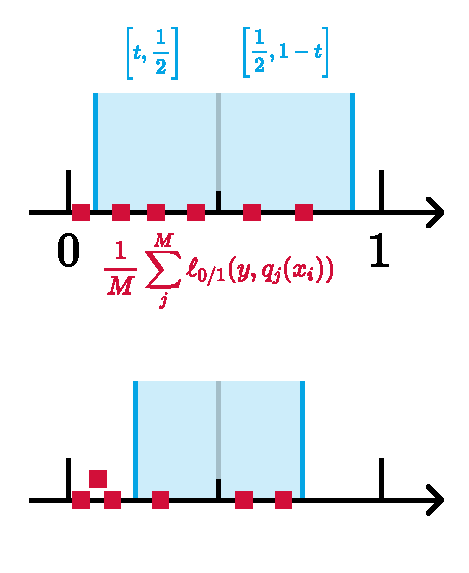
\includegraphics[width=\textwidth]{figma-illustrations/competence.pdf}
    \label{fig:competence}
    \caption{
        Illustration for the competence condition \ref{def:competence}. Red squares correspond to pairs $(X,Y)$ from the joint distribution of examples and outcomes. For each of these pairs, the average/expected member error $W_{\Theta}(X,Y) \approx \Mavg \Lzo(y, q_i)$ is the ratio of incorrect members. The center $\frac{1}{2}$ is the majority vote threshold. Informally, an ensemble is competent, if, for any two intervals defined by $t$ left and right of the threshold, more examples are in the left part. For the upper example, this holds. For the lower example, even though many examples are classified correctly by many members, the ensemble is \textit{not} competent.
        % TODO come back to this from persective of good/bad div
        % TODO emphasize that this is motivation for *dis*couraging disagreement on incorrect points (bad div)
    }
\end{marginfigure}
% TODO k-competence also shows rigorously how with larger k, there is less room for diversity
% TODO considerations of k-competence (namaly the thresholds) having an influence on weighting? I think so
% TODO this might also be a motivation for DRF approach
The weak learner assumption is a special case of this for $t = 0$.  % TODO Check
Ensembles of weak learners are competent and as such, this alternatively indirectly proves theorem \ref{thm:weak-learner-ensembles-nonnegative}.
% TODO elaborate, maybe star
 % TODO emphasize this insight

\begin{definition} (Competence, \cite{theisen}) An ensemble is competent iff
$$
\forall t \in \left[ 0, \frac{1}{2} \right]: ~ \prob{(X,Y) }{W(X,Y)  \in \left[ t, \frac{1}{2} \right]} ~ ~  \geq ~ ~ \prob{(X,Y) }{W(X,Y) \in \left[ \frac{1}{2}, 1-t \right]}
$$
\end{definition}
This assumption is used to show two results:
\begin{itemize}
	\item In competent ensembles, diversity-effect is non-negative.
	\sidenote{
		Although not acknowledging the role of diversity-effect as a component of the ensemble generalisation error and thus referring to it only as "ensemble improvement", one of the main results of \cite{theisen} is that, in competent ensembles, ensemble improvement (i.e. diversity-effect) is non-negative. 
	}
	\item bounds on the generalisation error (see \ref{later}) % TODO
\end{itemize}
The condition is illustrated in figure \ref{fig:competence}.  One can see that competence is essentially determined by the distribution of examples $(X,Y)$ over the range of $W(X,Y)$, divided by the majority vote threshold $\frac{1}{2}$. We have already seen that, similarly, diversity-effect in its apparent form of good and bad diversity is determined by just the same characteristics. How are these two related?

During the proof, which we will discuss in detail shortly, the following fact is established. Unless otherwise noted, all expectations and probabilites are over the distribution of $(X,Y)$.
$$
\text{ens. competent} ~\leftrightarrow~ \mathbb{E}_{}\left[ W~\ind{W < \frac{1}{2}} \right] \geq \mathbb{E}_{}\left[ 
\compl{W}~\ind{\compl{W} \leq \frac{1}{2} } 
\right] 
$$
We can rearrange this into a more suggestive form. Recall that $W = \mathbb{E}_{D, \Theta}\left[ \Lzo{Y}{q_{D,\Theta}(X)} \right]$. We now split off the expectation over $D$ and instead consider $W_{\Theta} = \mathbb{E}_{\Theta}\left[ \Lzo{Y}{q_{D, \Theta}(X)} \right]$. Rearranging the above and exploiting the linearity of expectation, we obtain
$$
d \defeq \mathbb{E}_{(X,Y),D }\left[ W_{\Theta} ~\ind{W_{\Theta} < \frac{1}{2}} \right]  - \mathbb{E}_{(X,Y) ,D}\left[ \compl{W_{\Theta}} ~\ind{\compl{W_{\Theta}} \leq \frac{1}{2} } \right] ~ ~ \geq ~ ~  0
$$
The indicator functions are mutually exclusive and can thus be understood as a case distinction. With slight abuse of notation, where the expectations are only over the subset of the distribution for which the case condition holds, we can write
$$
d = 
\begin{cases}
\mathbb{E}_{}\left[ W_{\Theta} \right] & \text{if~} W_{\Theta} < \frac{1}{2} \\[1em]
\mathbb{E}_{}\left[ \compl{W_{\Theta}}  \right]  = \mathbb{E}_{}\left[ 1 - W_{\Theta} \right]  & \text{if~} \compl{W_{\Theta}} \leq \frac{1}{2} 
\end{cases}
$$
For $k=2$, the cases of \ref{just-above} correspond directly to the cases of the ensemble being correct or incorrect of equation \ref{eq:binary-classification-cases}. Recalling the characterisation of good and bad diversity of lemma \ref{lemma-5.1.3}, we can see that $d$ is nothing else but the diversity-effect. 
Due to \ref{eq:binary-classification}, we can now see that for $k=2$, the other direction also holds: Any ensemble with non-negative diversity-effect also is competent. However, for $k>2$, this is not given: The plurality vote threshold is lower than $\frac{1}{2}$. There are ensembles which have non-negative diversity-effect (ensemble improvement) but are not competent. % TODO areas of wood23 fig20

% TODO use sth else than kappa or tildek, this is confusing
We will now proceed to argue that non-negative diversity-effect is in fact equivalent to a notion of confidence generalised to $k > 2$ classes. 
\begin{definition} $\star$ ($k$-competence) Let $\kappa \defeq 1 - \frac{1}{k}$. An ensemble is $k$-competent iff
$$
\forall t \in [0,1]:
\prob{(X,Y) }{W_{\rho} \in \left[ t, \kappa \right]}
\geq \prob{(X,Y) }{W_{\rho} \in \left[ 1-\kappa, 1-t \right]}
$$
\end{definition}
Competence as of definition \ref{def:competence} is $2$-competence.
\cite{theisen} only argued one direction: that competence implies non-negative diversity-effect. We now show that a very similar line of argument actually holds in both directions.
\begin{theorem} $\star$ Consider an ensemble for a $k$-class classification problem. Then
$$
\text{$k$-competence}  ~ ~ ~\leftrightarrow~ ~ ~  \text{diversity-effect} \geq 0
$$
\end{theorem}
% TODO himm, might be better to just use only lemma 2, not really sure why the rest is even needed
\begin{proof}
The approach is to show the inequality (see \ref{eq:gen-error-as-prob})
$$
\begin{align}
\mathbb{E}_{(X,Y),D }\left[ \Lzo{Y}{\bar{q}(X)} \right] &= \prob{}{Y \not= \bar{q}(X)} = \prob{(X,Y) ,D}{W_{\Theta} \geq \frac{1}{k}} \\
\leq \mathbb{E}_{(X,Y), D}\left[ W_{\Theta}  \right] 
\end{align}
$$
...
\end{proof}

----

% TODO somewhere, review that wood23 show that weak learner ens -> div-eff nonnegative
% In other settings, however, we are mainly concerned with whether the correct class is assigned or not. This gives rise to the \zeroone-loss $\ell(y', y) \defeq \mathbb{1}\left[ y' \not = y \right]$. 
% % The expected loss of a model $q$ is $\ell(q_{}) \defeq \mathbb{E}_{D}\left[ \Lzo{q_{}(X)}{Y} \right]$. Let $\bar{q}$ be the majority vote combiner.
% In the following, we will review results which characterise the ensemble improvement in this setting.

% Given ensemble members $q_{\Theta}$ parameterised by a random variable $\Theta$, denote the proportion of erroneous ("wrong") classifiers for an example-outcome pair $(X,Y)$ as $W_{\Theta} \defeq W_{\Theta}(X,Y) \defeq \mathbb{E}_{\Theta}\left[ \Lzo{q_{\Theta}(X)}{Y} \right]$. This expectation is approximated by the average member loss $\Mavg\Lzo{q_{i}(X)}{Y}$. 

% \begin{definition}
% In the statistical setting, if an ensemble member is constructed according to parameters $\Theta$, we write
% $$
% W_{\Theta}(X,Y) \defeq \mathbb{E}_{\Theta}\left[ \Lzo{Y}{q_{\Theta}(X)} \right] 
% $$
% If a concrete ensemble of members $q_{1}, \dots, q_{M}$ is given, we write
% $$
% \Wmem(X,Y) \defeq \Mavg \Lzo{Y}{q_{i}(X)}
% $$
% As with other variables, we sometimes omit explicitly stating the dependence on $(X,Y)$. 
% \end{definition}

A common idea is that, in order for ensembling to be effective, the performance of individual members must not be too bad. In the remainder of this section, we will review some assumptions that imply ensemble effectivity and show that they are in fact tightly related.

% !! TODO check 
\begin{definition} 
    % TODO relate to margin defs
    % TODO cite
   \label{def:weak-learner}  (Weak learner)
    need to check / reformulate this
    % A model $q_\Theta$ is a \textit{weak learner} iff it performs better than as if randomly guessing, i.e. 
    % $$\mathbb{E}_{(X,Y)}\left[ W_{\Theta}(X,Y) \right] \geq \frac{1}{2}$$.
\end{definition}

\begin{theorem} 
    \label{thm:weak-learner-ensembles-nonnegative}
    (\cite{wood23}) In an ensemble of weak learners, diversity-effect is non-negative:
$$
% TODO notation
\mathbb{E}_{D}\left[ 
\mathbb{E}_{Y}\left[ 
\Mavg \Lzo{Y}{q_{i}} - \Lzo{Y}{\bar{q}}
\right] 
\right] 
~ ~ \geq ~ ~ 0
$$
\end{theorem}
% TODO at least provide intuition on why that is
\begin{proof}
... essentially using jury theorem
\end{proof}

% TODO double terms (diversity-effect and ensemble improvement), this is confusing, they're really the same thing.

However, this is not a sufficient 
% todo check wording of "sufficient"
condition, as example \ref{fig:pathological-example} shows.
%


---

% TODO the below needs to be reintegrated
 The competence assumption, however, allows to exclude pathological cases 
 
 and give tighter bounds for the ensemble improvement -- here in terms of disagreements between members.
\sidenote{
    Because we focus mainly on binary classification, we give this result in its simplified form for $k=2$ classes but note that their actual result gives bounds for arbitrary $k$.
}
% TODO really need to resolve the naming conflict ensemble improvement / diversity / ambiguity
% TODO overfull
\begin{theorem} (\cite{theisen}, for binary classification) Let $D(q_{\Theta}, q_{\Theta'}) \defeq \mathbb{E}_{D}\left[ \Lzo{q_{\Theta}}{q_{\Theta'}} \right]$ be the \textit{disagreement rate} between two members. In competent ensembles it holds that
$$
\mathbb{E}_{\Theta, \Theta'}\left[ D(q_{\Theta}, q_{\Theta'}) \right] 
~ ~  \geq ~ ~ 
\mathbb{E}_{\Theta}\left[ L(q_{\Theta}) - L(\bar{q}) \right] 
~ ~  \geq ~ ~ 
\mathbb{E}_{\Theta, \Theta'}\left[ D(q_{\Theta}, q_{\Theta'}) \right] - \mathbb{E}_{\Theta}\left[ L(q_{\Theta}) \right]  
$$
\end{theorem}

% TODO this was really important to put here for some reason but now I lost my train of thought....
% -- I guess it was that competence is actually motivation for DRF weightin
% in the sense that it would influence margins/ratio incorrect trees st the ensemble is "more competent"
% TODO should show how this improves upon the naive bound above
% TODO mention that we can (easily) experimentally verify that RFs are competent

% TODO at least can relate this to other bounds...

% TODO should also at least mention margin bounds, breiman bound...

% TODO for more, cf louppe 4.1.2


\end{document}